\documentclass[../the.tex]{subfiles}
\begin{document}

Trong phạm vi nghiên cứu này sẽ sử dụng mô hình Yolov7, Yolov8, SSD MobiNet và FasterRCNN. Mục \ref{sec:model} giới thiệu về các mô hình được sử dụng. Mục \ref{sec:dataset} mô tả về tập dữ liệu, và phương pháp đánh giá mô hình được trình bày trong Mục \ref{sec:eval}

\section{Tập dữ liệu}
\label{sec:dataset}

{\fontsize{13}{12} \selectfont
	Trong phạm vi nghiên cứu, các tập dữ liệu sử dụng sẽ là TrashNet \cite{yang2016classification}, Taco \cite{proença2020taco} và bổ sung tập dữ liệu tự thu thập được ở ĐBSCL.
	Tham khảo việc phân loại rác của Yan \cite{yang2016classification} và quá trình thu thập dữ liệu thực tế nhận thấy các loại rác bằng thủy tinh ở môi trường bên ngoài rất thường là các mảnh kính trong suốt nhìn thấy nên hoặc có độ phản chiếu ánh sáng cao nên rất khó phát hiện, vì vậy các thủy tinh sẽ được gom vào các loại rác khác.
	Các giấy và thùng giấy sẽ được gom lại vì cùng chất liệu. Cuối cùng mô hình sẽ phân các loại ra làm các lớp:
	\begin{itemize}
		\item Kim loại gồm chủ yếu là các nắp bia, các vỏ bình làm bằng kim loại.
		\item Nhựa - nilon rất phổ biến, gồm các vật liệu làm từ nhựa như ly nhựa, các túi nilon.
		\item Giấy gồm các vật liệu từ giấy, các thùng giấy, vỏ gói thuốc lá, hộp giấy.
		\item Rác khác là các loại rác còn lại với từng loại xuất hiện ít hoặc khó phát hiện như thủy tinh, các vỏ gói đa sắc,
		      mút, vải,\dots
	\end{itemize}

\subsection{TrashNet}
\label{sec:trashnet}
	{\fontsize{13}{12} \selectfont
		TrashNet là tập dữ liệu đươc giới thiệu trong bài nghiên cứu của \cite{yang2016classification} bao gồm các lớp và số lượng như bảng \ref{tab:dataset}. Tất cả hình ảnh được chụp bằng điện thoại Iphone7 sử dụng ánh sáng mặt trời hoặc ánh sáng phòng, các đối tượng được chụp trong nền trắng hoặc bao quát toàn bộ khung hình, một số hình ảnh ở tập Trashnet ở hình
		\ref{fig:dataset_0}.
		Do mục đích ban đầu của tập dữ liệu dùng để phân lớp nên nghiên cứu phải thực hiện gán hộp giới hạn cho bộ dữ liệu để phù hợp với nhu cầu phát hiện đối tượng. Tập dữ liệu TrashNet bao gồm các đối tượng có kích thước lớn và rõ ràng, mục đích sử dụng tăng độ nhận dạng cho mô hình. Bảng \ref{tab:dataset1} thể hiện số lượng đối tượng sau khi đã gán hộp giới hạn cho tập dữ liệu, hình
		\ref{fig:dataset_1} giói thiệu tập dữ liệu khi có hộp.
	}
}

\begin{table}[!ht]
	\centering
	\caption{Thuộc tính của tập dữ liệu TrashNet}
	\begin{tabular}{|p{2cm}|p{4cm}|p{3.5cm}|p{2cm}|}
		\hline
		\multicolumn{1}{|l|}{
			\textbf{\#}}
		 & \multicolumn{1}{c|}{\textbf{Lớp}}
		 & \multicolumn{1}{c|}{\textbf{Số lượng ảnh}} \\
		\hline

		1
		 & Cardboard
		 & 403                                        \\
		\hline

		2
		 & Paper
		 & 594                                        \\
		\hline

		3
		 & Glass
		 & 501                                        \\
		\hline

		4
		 & Plastic
		 & 482                                        \\
		\hline

		5
		 & Metal
		 & 410                                        \\
		\hline

		6
		 & Trash
		 & 137                                        \\
		\hline


		\textbf{Tổng cộng}
		 &
		 & 2524                                       \\
		\hline
	\end{tabular}

	\label{tab:dataset}
\end{table}

\begin{figure}[H]
	\centering
	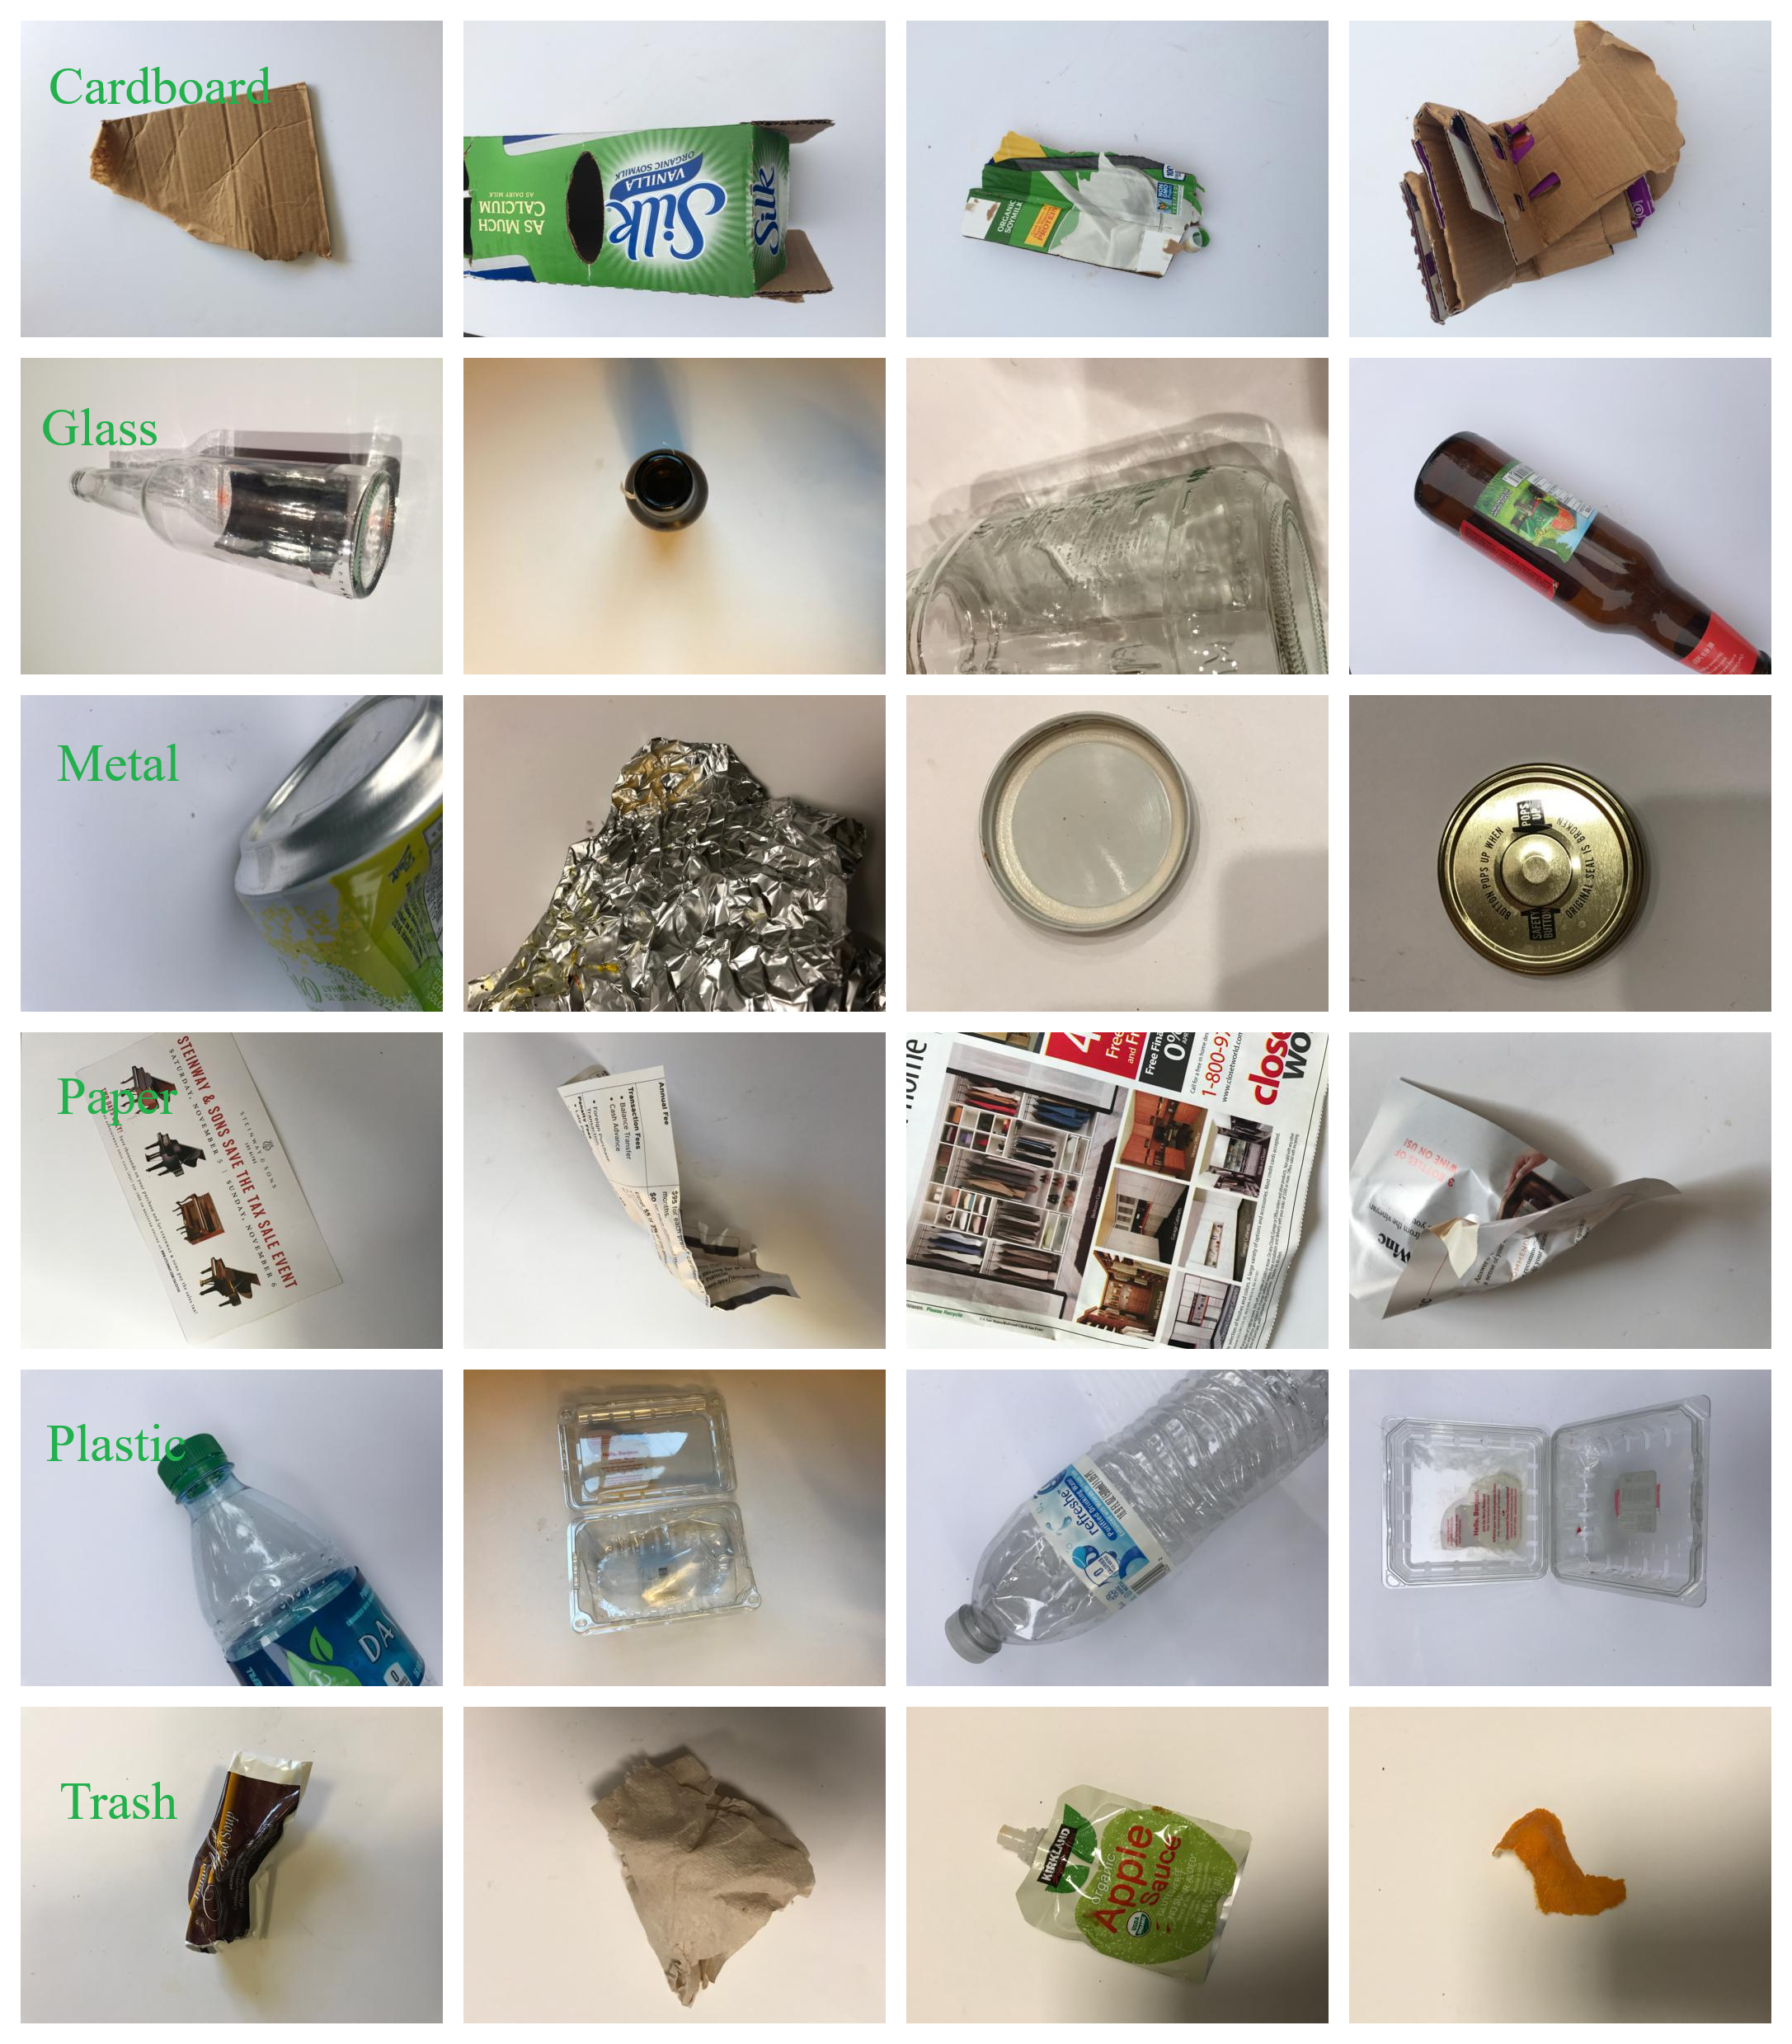
\includegraphics[width=1\textwidth]{trashnet_sample.png}
	\caption{Ví dụ về hình ảnh của tập dữ liệu TrashNet}
	\label{fig:dataset_0}
\end{figure}

\begin{table}[!ht]
	\centering
	\caption{Thuộc tính của tập dữ liệu TrashNet khi được gán hộp giới hạn}
	\begin{tabular}{|p{2cm}|p{4cm}|p{3.5cm}|p{2cm}|}
		\hline
		\multicolumn{1}{|l|}{
			\textbf{\#}}
		 & \multicolumn{1}{c|}{\textbf{Lớp}}
		 & \multicolumn{1}{c|}{\textbf{Số lượng vật thể}} \\
		\hline

		1
		 & Cardboard
		 & 404                                            \\
		\hline

		2
		 & Paper
		 & 601                                            \\
		\hline

		3
		 & Glass
		 & 509                                            \\
		\hline

		4
		 & Plastic
		 & 479                                            \\
		\hline

		5
		 & Metal
		 & 410                                            \\
		\hline

		6
		 & Trash
		 & 149                                            \\
		\hline


		\textbf{Tổng cộng}
		 &
		 & 2552                                           \\
		\hline
	\end{tabular}

	\label{tab:dataset1}
\end{table}


\begin{figure}[H]
	\centering
	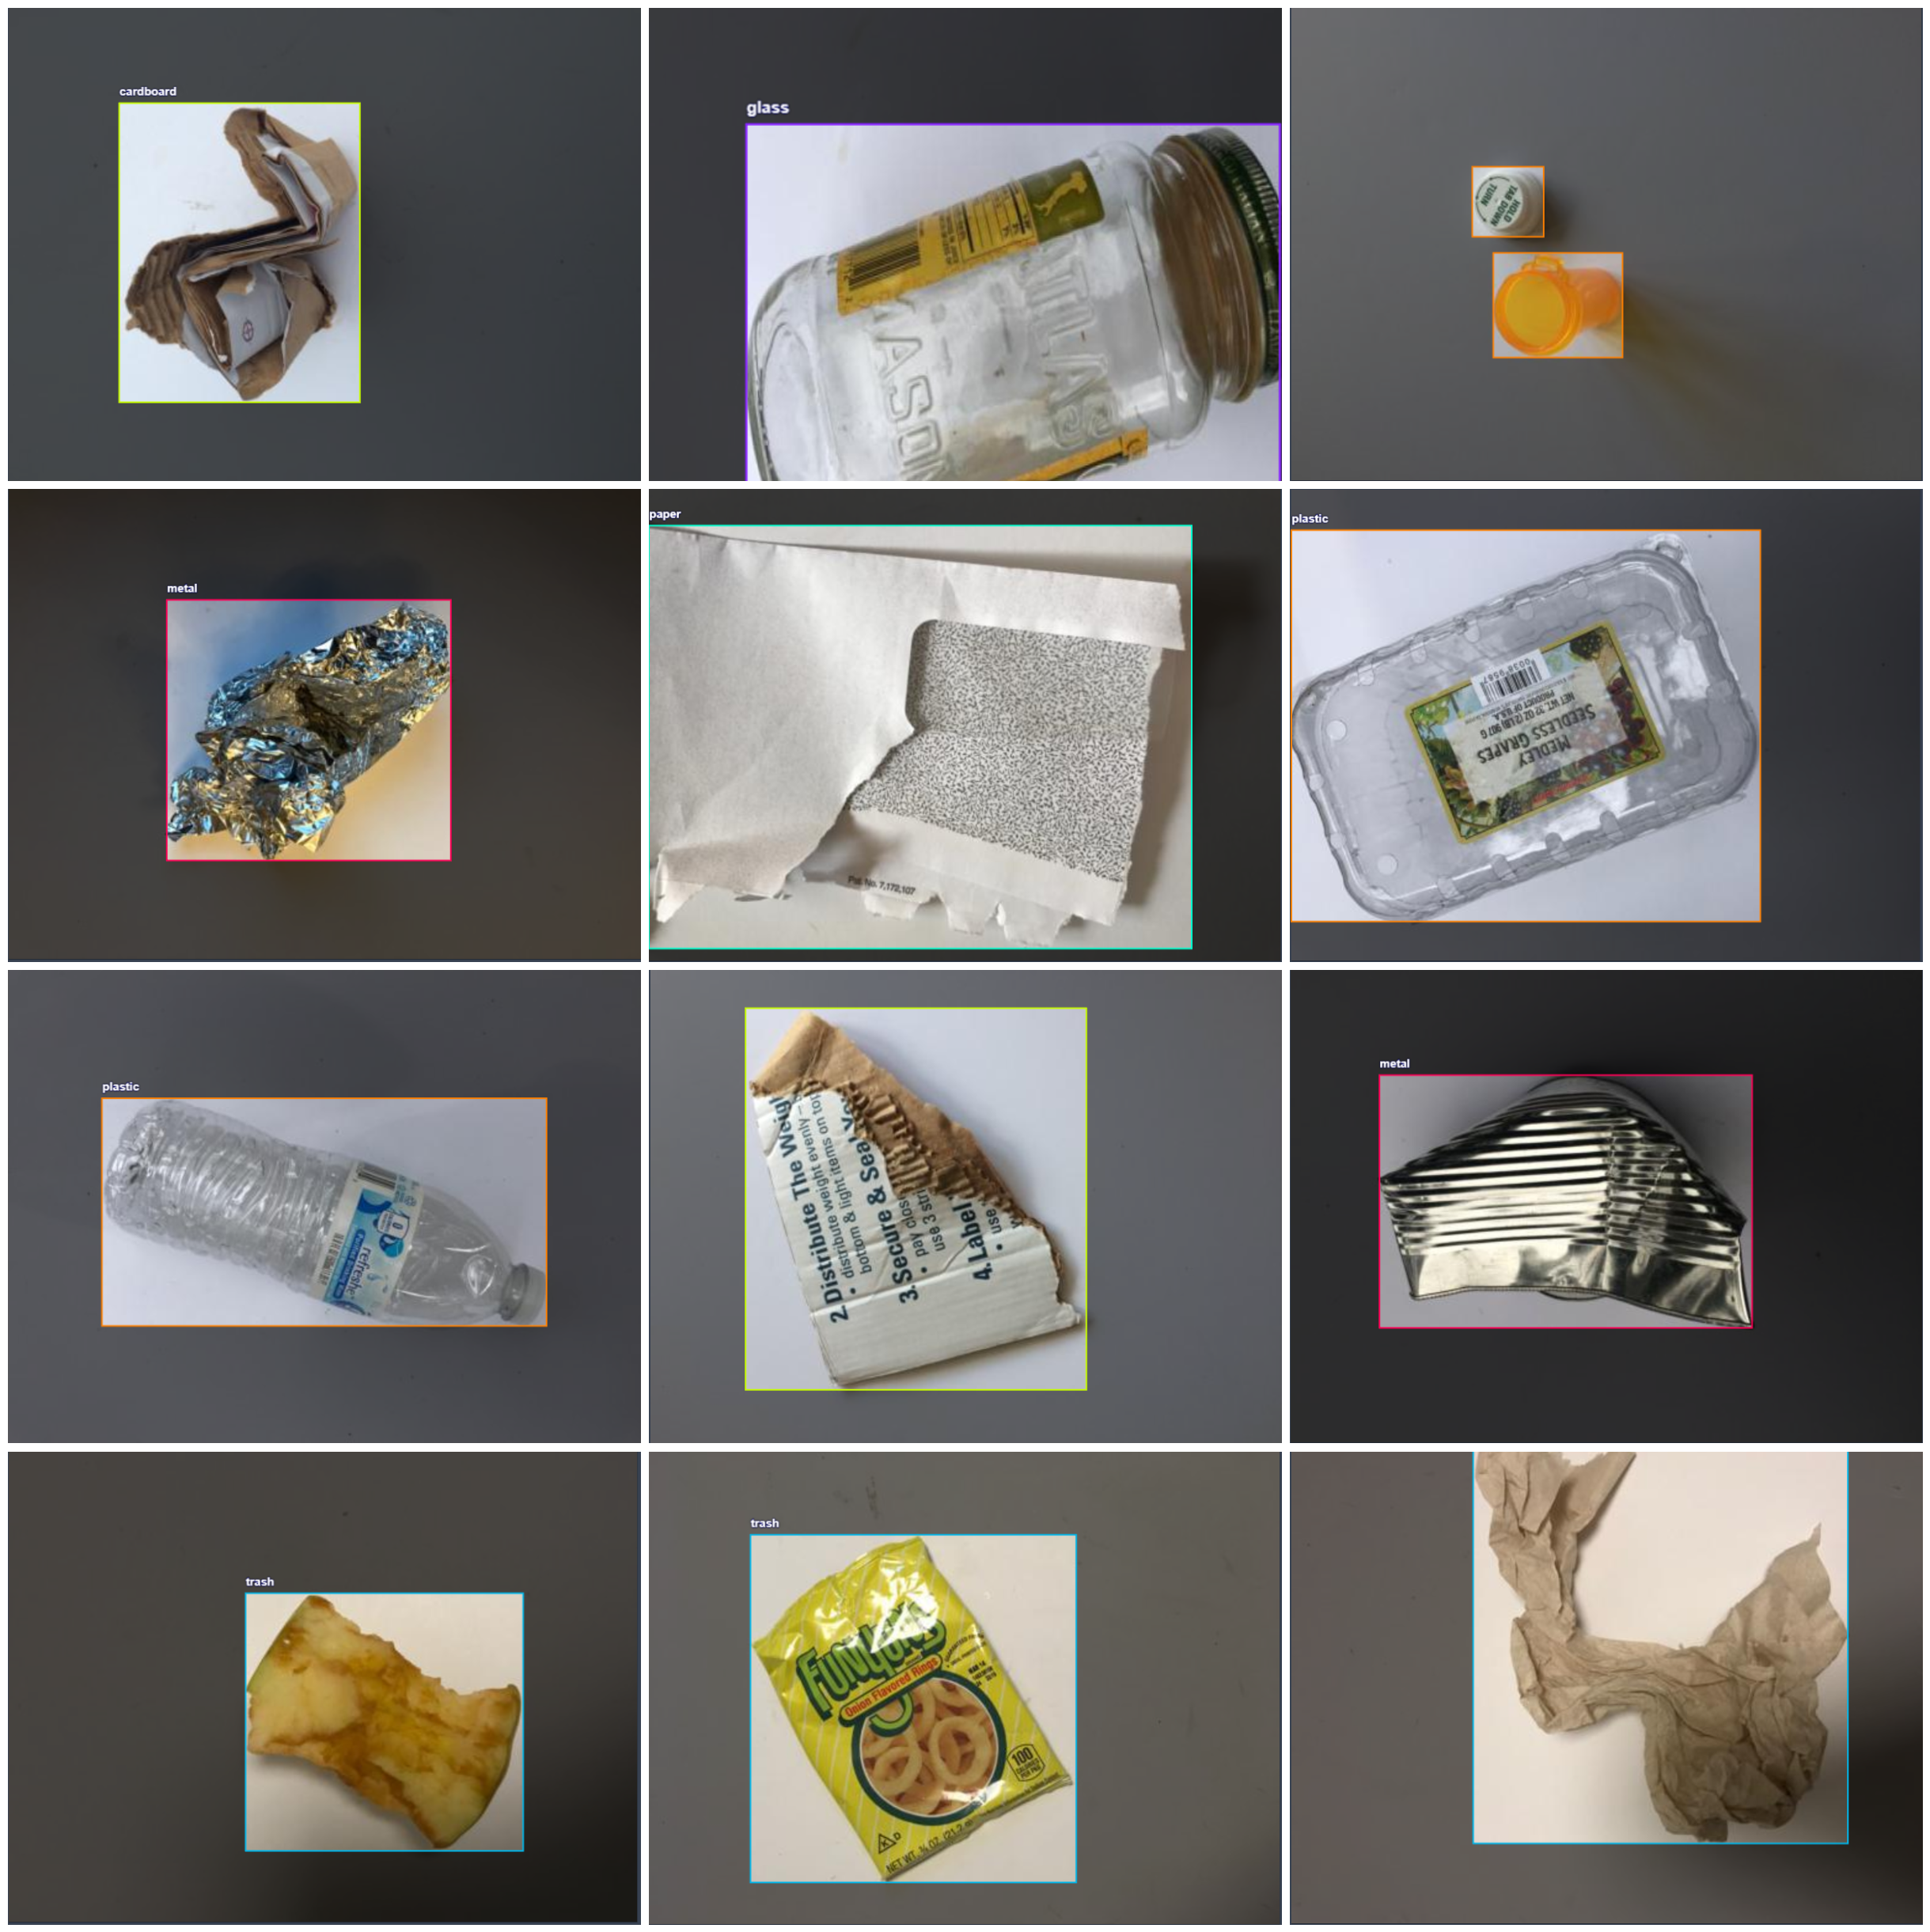
\includegraphics[width=1\textwidth]{trashnet_sample2.png}
	\caption{Ví dụ về hình ảnh của tập dữ liệu TrashNet được gán hộp giới hạn}
	\label{fig:dataset_1}
\end{figure}



\subsection{Taco}
\label{sec:Taco}
{\fontsize{13}{12} \selectfont
	Taco là một tập dữ liệu hình ảnh mở về chất thải trong tự nhiên. Tập dữ liệu chứa các hình ảnh về rác được chụp trong nhiều môi trường khác nhau, từ những bãi biển đến đường phố London. Những hình ảnh này được gắn nhãn và phân đoạn thủ công để đào tạo và đánh giá các thuật toán phát hiện đối tượng.
	Bộ dữ liệu được cung cấp
	theo chuẩn json của COCO. Hiện tại bộ dữ liệu có 1.500 ảnh với 4.784 vật thể
	và 3918 ảnh mới cần được gán nhãn.
}

\begin{figure}[H]
	\centering
	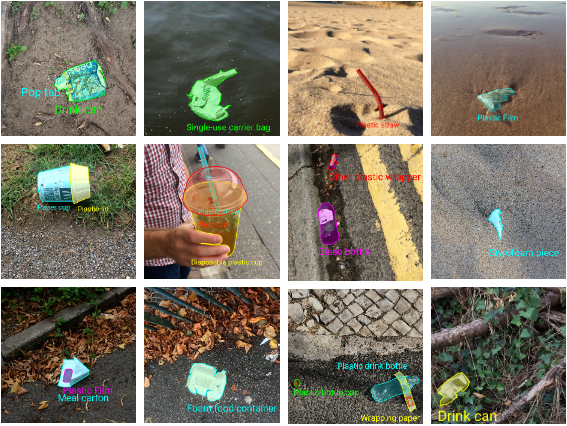
\includegraphics[width=1\textwidth]{Taco.png}
	\caption{Ví dụ về bộ dữ liệu Taco \cite{proença2020taco}}
	\label{fig:dataset_taco}
\end{figure}
{\fontsize{13}{12} \selectfont

Bộ dữ liệu gồm 28 danh mục lớn  (Hình \ref{fig:dataset_taco_1_a}) và 60 danh mục nhỏ (Hình \ref{fig:dataset_taco_1_b}) với
6 loại nền là rác, thảm cỏ, nước, trong nhà, vỉa hè, cát đá (Hình \ref{fig:dataset_taco_1_c}). Do
điều kiện đường phố ở một số tỉnh ĐBSCL nên nghiên cứu loại bỏ ngữ cảnh trong nhà, cát đá và nước phục vụ cho mục đích huấn luyện mô hình. Các danh
mục nhỏ được gom nhóm phù hợp thành bốn loại rác đề ra của nghiên cứu như Bảng \ref{tab:taco_map}. Bộ dữ liệu Taco thể hiện sự đa dạng trong từng loại rác,
tuy nhiên đó cũng là sự hạn chế khi có những lớp có quá ít dữ liệu như Carded blister pack (1 đối tượng), Battery (2 đối tượng), và các lớp có quá nhiều đối tượng như Cigarette (667 đối tượng) và Unlabeled litter (516 đối tượng).
}

\begin{figure}[H]	
	\centering
	\subfloat[\centering {\fontsize{11}{10} \selectfont Danh mục lớn }]{{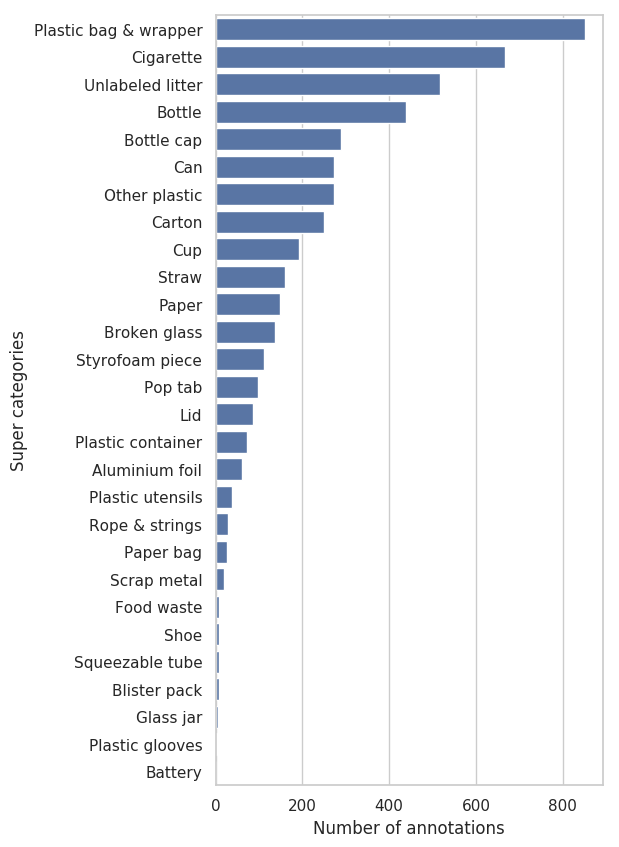
\includegraphics[width=7cm]{taco_super.png} \label{fig:dataset_taco_1_a}}}%
	\qquad
	\subfloat[\centering {\fontsize{11}{10} \selectfont Danh mục nhỏ}]{{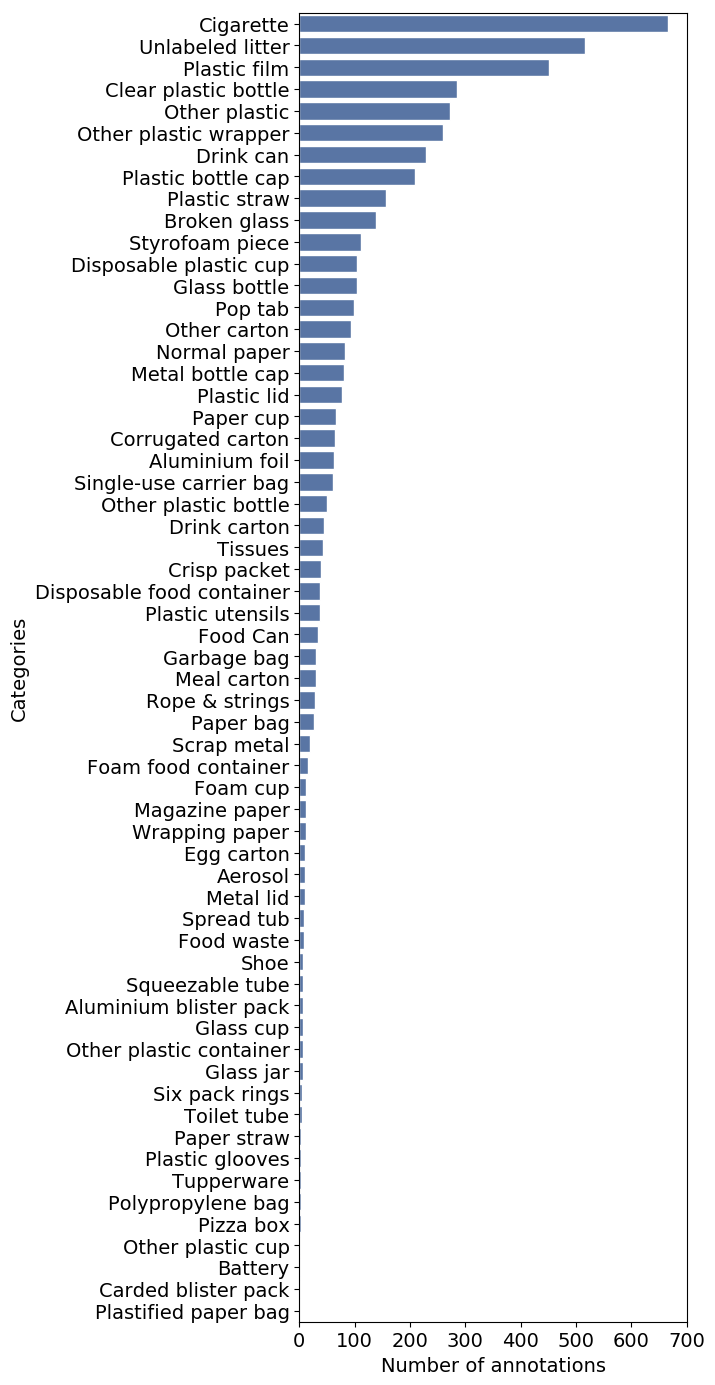
\includegraphics[width=7cm]{taco_cat.png} \label{fig:dataset_taco_1_b}}}%
	\qquad
	\subfloat[\centering {\fontsize{11}{10} \selectfont Tỉ lệ nền}]{{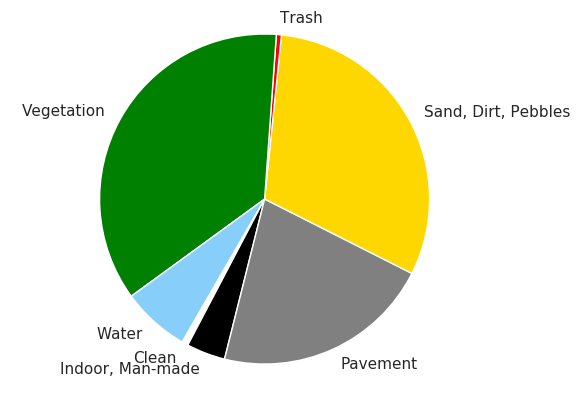
\includegraphics[width=10cm]{taco_bg.png} \label{fig:dataset_taco_1_c}}}%
	\caption{Thống kê bộ dữ liệu Taco}%
	\label{fig:dataset_taco_1}
\end{figure}

\begin{table}[!ht]
    \centering
    \caption{Bảng chuyển các lớp của Taco sang lớp của mô hình}
    \begin{tabular}{|l|l|l|l|}
		\hline 
		 \multicolumn{1}{|c|}{\textbf{Taco}}
		 & \multicolumn{1}{c|}{\textbf{Mô hình}}
		 & \multicolumn{1}{c|}{\textbf{Taco}}
		 & \multicolumn{1}{c|}{\textbf{Mô hình}}  \\
		\hline
        Aluminium foil & kim\_loai & Magazine paper & giay \\ \hline
        Battery & kim\_loai & Tissues & giay \\ \hline
        Aluminium blister pack & khac & Wrapping paper & giay \\ \hline
        Carded blister pack & khac & Normal paper & giay \\ \hline
        Other plastic bottle & nhua\_nilon & Paper bag & giay \\ \hline
        Clear plastic bottle & nhua\_nilon & Plastified paper bag & giay \\ \hline
        Glass bottle & khac & Plastic film & nhua\_nilon \\ \hline
        Plastic bottle cap & nhua\_nilon & Six pack rings & khac \\ \hline
        Metal bottle cap & kim\_loai & Garbage bag & nhua\_nilon \\ \hline
        Broken glass & khac & Other plastic wrapper & nhua\_nilon \\ \hline
        Food Can & kim\_loai & Single-use carrier bag & nhua\_nilon \\ \hline
        Aerosol & kim\_loai & Polypropylene bag & nhua\_nilon \\ \hline
        Drink can & kim\_loai & Crisp packet & khac \\ \hline
        Toilet tube & giay & Spread tub & nhua\_nilon \\ \hline
        Other carton & giay & Tupperware & nhua\_nilon \\ \hline
        Egg carton & giay & Disposable food container & nhua\_nilon \\ \hline
        Drink carton & giay & Foam food container & giay \\ \hline
        Corrugated carton & giay & Other plastic container & nhua\_nilon \\ \hline
        Meal carton & giay & Plastic glooves & nhua\_nilon \\ \hline
        Pizza box & giay & Plastic utensils & nhua\_nilon \\ \hline
        Paper cup & giay & Pop tab & kim\_loai \\ \hline
        Disposable plastic cup & nhua\_nilon & Rope \& strings & khac \\ \hline
        Foam cup & giay & Scrap metal & kim\_loai \\ \hline
        Glass cup & khac & Shoe & khac \\ \hline
        Other plastic cup & nhua\_nilon & Squeezable tube & khac \\ \hline
        Food waste & khac & Plastic straw & nhua\_nilon \\ \hline
        Glass jar & khac & Paper straw & nhua\_nilon \\ \hline
        Plastic lid & nhua\_nilon & Styrofoam piece & khac \\ \hline
        Metal lid & kim\_loai & Unlabeled litter & khac \\ \hline
        Other plastic & nhua\_nilon & Cigarette & khac \\ \hline
    \end{tabular}
	\label{tab:taco_map}
\end{table}
\subsection{Dữ liệu tự thu thập}
\label{sec:own}
{\fontsize{13}{12} \selectfont
Hình \ref{fig:dataset_own} là bộ dữ liệu được thực hiện lấy mẫu ở các tỉnh thành ở ĐBSCL như Cần Thơ, Vĩnh Long và chủ yếu ở Trà Vinh nhầm phản ánh thực tế tình trạng rác ở địa phương. 
Dữ liệu thu thập gồm 663 hình ảnh với 1766 đối tượng được chia cho bốn lớp kim loại, nhựa - nilon, giấy, rác khác với trung bình 2.6 đối tượng mỗi hình ảnh (bảng \ref{tab:datasetown}).
Phần lớn là các hộp thức ăn giấy, các bọc nilon, ly nhựa, túi rác, khẩu trang giấy và các phần rác cũ không có hình dạng cố định. 
Việc thu thập thêm dữ liệu nhầm giúp mô hình học tập và cải thiện khả năng phát hiện đúng thực tế. Trong quá trình thực hiện thu thập dữ liệu gặp những vấn đề như sau:
\begin{itemize}
	\item Các rác chồng chéo khó xác định hộp giới hạn.
	\item Tình trạng các rác cũ, rác nhỏ bị ẩn vào nền, rất khó xác định nhãn.
	\item Xuất hiện các đối tượng rác có thể gồm nhiều nhãn. Ví dụ như túi nilon chứa bọc giấy, lon kim loại, các gói sắc nét hộp thức ăn nhựa trong suốt chứa rác hữu cơ.
	\item Phần rác kim loại xuất hiện ít, vì hầu hết được người dân xử lí chủ động trước. Tuy nhiên phần rác kim loại vẫn có đặc tính dễ phát hiện và bổ sung dữ liệu từ Taco \cite{proença2020taco} và TrashNet.
	\item Các loại còn lại được gom vào rác khác sẽ giảm khả năng phân lớp vì độ đa dạng cao.
\end{itemize}

\bigskip
}
{\fontsize{13}{12} \selectfont
\begin{table}[!ht]
	\centering
	\caption{Thuộc tính của tập dữ liệu tự thu thập}
	\begin{tabular}{|l|l|l|l|}
		\hline
		 \multicolumn{1}{|c|}{\textbf{Lớp}}
		 & \multicolumn{1}{c|}{\textbf{Số hình}} 
		 & \multicolumn{1}{c|}{\textbf{Số vật thể}}
		 & \multicolumn{1}{c|}{\textbf{Tỉ lệ}}
		  \\
		\hline

		  Nhựa - Nilon & 392 & 761 & 43.1\%  \\
		\hline

			Giấy & 339 & 552   & 31.3\%                                        \\
		\hline

		 Rác khác & 209 & 350   & 19,8\%                                        \\
		\hline

		 Kim loại & 60 & 103    & 5,8\%                                         \\
		\hline
		 Ảnh không vật thể & 200 & 0   & 0                                         \\
		\hline

	\end{tabular}

	\label{tab:datasetown}
\end{table}
Bảng \ref{tab:datasetown} thể hiện các rác thải nhựa-nilon chiếm phần lớn các loại rác ở đường phố hiện nay và các rác kim loại rất ít chỉ khoảng 5,8\% dữ liệu thu thập được.
Việc mất cân bằng dữ liệu ở tập dữ liệu tự thu thập sẽ được bổ sung bằng các tập dữ liệu của Taco và TrashNet, từ đó tạo ra bộ dữ liệu để huấn luyện và kiểm thử.
Ngoài ra nghiên cứu còn thu thập thêm 200 hình ảnh nền để tăng cường dữ liệu, đặt ra vấn đề các ảnh nền không chứa đối tượng nào (background) có tăng khả năng nhận diện của mô hình bằng cách giảm việc nhận dạng sai các đối tượng không phải là rác hay không.
}


\begin{figure}[H]
	\centering
	\includegraphics[width=1\textwidth]{data_own.png}
	\caption{Ví dụ về bộ dữ liệu thu thập}
	\label{fig:dataset_own}
\end{figure}

\subsection{Dữ liệu sử dụng cho mô hình}
{\fontsize{13}{12} \selectfont 
Trong phạm vi nghiên cứu sẽ sử dụng kết hợp giữa các bộ dữ liệu được nêu ở mục \ref{sec:trashnet}, \ref{sec:Taco}, \ref{sec:own} để tạo ra các bộ dữ liệu phù hợp với các mục đích huấn luyện.
Nghiên cứu ban đầu sẽ tìm ra mô hình phù hợp với phát hiện rác, sau đó sẽ đề xuất điều chỉnh các thông số và bổ sung dữ liệu nền để cải thiện mô hình.
Bảng \ref{tab:datasetmain} trình bày sự kết hợp của cả ba bộ dữ liệu. 
}
\begin{table}[!ht]
	\centering
	\caption{Thuộc tính của tập dữ liệu của nghiên cứu}
	\begin{tabular}{|c|c|c|c|c|ccccc}
	\cline{1-5}
	\textbf{Lớp}                           &            & \textbf{TrashNet} & \textbf{Taco} & \textbf{Thu thập} &  &  &  &  &  \\ \cline{1-5}
	\multirow{2}{*}{\textbf{Nhựa - nilon}} & Hình ảnh   & 495               & 604           & 392               &  &  &  &  &  \\ \cline{2-5}
										   & Đối tượng  & 496               & 1252          & 761               &  &  &  &  &  \\ \cline{1-5}
	\multirow{2}{*}{\textbf{Giấy}}         & Hình ảnh   & 591               & 349           & 339               &  &  &  &  &  \\ \cline{2-5}
										   & Đối tượng  & 591               & 488           & 552               &  &  &  &  &  \\ \cline{1-5}
	\multirow{2}{*}{\textbf{Kim loại}}   & Hình ảnh   & 409               & 221           & 60                &  &  &  &  &  \\ \cline{2-5}
										   & Đối tượng  & 410               & 346           & 103               &  &  &  &  &  \\ \cline{1-5}
	\multirow{2}{*}{\textbf{Rác khác}}     & Hình   ảnh & 587               & 365           & 209               &  &  &  &  &  \\ \cline{2-5}
										   & Đối tượng  & 612               & 547           & 350               &  &  &  &  &  \\ \cline{1-5}
	\end{tabular}
	\label{tab:datasetmain}
\end{table}

{\fontsize{13}{12} \selectfont
Nghiên cứu sẽ sử dụng các bộ dữ liệu như sau:
\begin{itemize}
	\item Bộ dữ liệu \#1 kết hợp của dữ liệu Taco và tự thu thập gồm một lớp là rác, giúp đánh giá và chọn ra mô hình phù hợp trong các mô hình phát hiện đối tượng một giai đoạn.
	\item Bộ dữ liệu \#2 kết hợp của dữ liệu Taco, tự thu thập và bổ sung dữ liệu TrashNet để giải quyết vấn đề mất cân bằng dữ liệu. 
	Trong đó, lớp "Unlabeled litter" của bộ dữ liệu Taco sẽ được gán lại nhãn thủ công để phù hợp với dữ liệu của nghiên cứu. Bảng \ref{tab:datasetmain} mô tả chi tiết các hình ảnh và đối tượng được sử dụng trong nghiên cứu được lấy từ việc kết hợp ba bộ dữ liệu.\label{item:dataset}
	\item Bộ dữ liệu \#2 nhưng bổ sung 200 hình nền không có đối tượng.
\end{itemize}
\bigskip

Tóm lại việc gán nhãn cho dữ liệu ảnh hưởng đến mô hình rất nhiều, vì rất dễ nhầm lẫn về định nghĩa rác theo thành phần từ các lớp của bộ dữ liệu Taco (bảng \ref{tab:taco_map}).
Ngoài ra bộ dữ liệu Taco là do cộng đồng đóng góp, vì vậy việc xuất hiện nhiều lớp "Unlabeled litter" sẽ gây nhiễu cho dữ liệu, cần phải gán nhãn lại.
Tập dữ liệu để đánh giá mô hình ở bộ dữ liệu \#2 và \#3 sẽ chỉ gồm dữ liệu của \ref{sec:Taco} và \ref{sec:own} để đánh giá khả năng phát hiện thực tế của mô hình.
}
% Please add the following required packages to your document preamble:
% \usepackage{multirow}
% Please add the following required packages to your document preamble:
% \usepackage{multirow}


{\fontsize{13}{12} \selectfont  }
\section{Các mô hình sử dụng}
\label{sec:eval}



\subsection{Các chỉ số để so sánh hiệu năng}

{\fontsize{13}{12} \selectfont
	Độ chính xác của mô hình phát hiện gãy xương được xác định bởi chất lượng của việc khoanh vùng và phân loại đối tượng. Trong nghiên cứu này sử dụng các độ đo: độ chính xác, độ nhạy, F$_1$ và AUC-ROC. Ngoài ra, so sánh giữa giá trị dự đoán và nhãn để xác định vùng gãy xương, nghiên cứu cũng sử dụng độ đo IoU (Intersection over Union).
}

\subsubsection*{Độ chính xác, độ nhạy và F$_1$}

{\fontsize{13}{12} \selectfont
	Xét các định nghĩa sau:
	\begin {itemize}
	\item True Positive (TP) thể hiện những giá trị dự đoán chính xác gãy xương.
	\item True Negative (TN) thể hiện các dự đoán chính xác không gãy xương.
	\item False Positive (FP) thể hiện các dự đoán nhầm về không gãy xương.
	\item False Negative (FN) thể hiện các dự đoán nhầm về gãy xương.
	\end {itemize}

	Công thức toán học của Precision và Recall được thể hiện lần lượt theo Công thức \ref{eq:precision} và Công thức \ref{eq:recall}. Precision và Recall có ý nghĩa khác nhau trong bài toán phát hiện đối tượng. Trong trường hợp muốn phát hiện nhiều đối tượng trong ảnh, chúng ta cần quan tâm đến giá trị Recall. Ngược lại, nếu muốn phát đối tượng chính xác hơn, ta nên cố gắng làm cho giá trị Precision càng lớn càng tốt. Do đó, hai giá trị này bị ràng buộc lẫn nhau. Điều đó có nghĩa là, khi giá tị Recall tăng lên, Precision sẽ giảm lại và ngược lại. Ngoài ra, giá trị F$_1$ là mức trung bình hài hòa giữa Precision và Recall (như trong Công thức \ref{eq:f1}).
}

\begin{equation}
	Precision = \frac{TP}{TP + FP}
	\label{eq:precision}
\end{equation}

\begin{equation}
	Recall = \frac{TP}{TP + FN}
	\label{eq:recall}
\end{equation}

\begin{equation}
	F_1 = 2 \times \frac{Precision \times Recall}{Precision + Recall} = \frac{2TP}{2TP + FP + FN}
	\label{eq:f1}
\end{equation}

\subsubsection*{IoU}

{\fontsize{13}{12} \selectfont
	Số liệu IoU đo lường mức độ chính xác của một hộp giới hạn được dự đoán so với nhãn thật sự.

	Hình chữ nhật phía trên bên trái là nhãn và hình chữ nhật phía dưới bên phải là phần dự đoán. Vì kết quả phát hiện luôn khác với nhãn, IoU được xác định bằng cách chia giao điểm của phần dự đoán và nhãn cho phần kết hợp của chúng. Trong Yolo, ngưỡng IoU luôn được đặt là 0.5. Có nghĩa là, khi giá trị IoU của kết quả phát hiện lớn hơn 0.5, nó sẽ được coi là một TP. Khi giá trị IoU của kết quả phát hiện nhỏ hơn 0.5, nó sẽ được coi là một TN. Bằng cách điều chỉnh ngưỡng IoU, chúng ta có thể kiểm soát tỷ lệ TP và TN.
}

\begin{figure}[ht!]
	\centering
	\includegraphics[width=1\textwidth]{images/IoU.PNG}
	\caption{Định nghĩa của IoU}
	\label{fig:IoU}
\end{figure}

\subsubsection*{Thử nghiệm McNemar}

Thử nghiệm McNemar \cite{McNemar1947} là một thử nghiệm đối với dữ liệu được ghép nối, như trong trường hợp bảng dự phòng $2 \times 2$ có đặc điểm lưỡng phân. Thử nghiệm McNemar xác định xem tần số hàng và cột biên có bằng nhau hay không, còn được gọi là tính đồng nhất biên. Thử nghiệm McNemar được thiết kế để tập trung chủ yếu vào sự khác biệt giữa hai mô hình, cụ thể là mỗi mô hình có thể sẽ cho một kết quả dự đoán khác nhau trên cùng dữ liệu đầu vào . Xét bảng dự phòng $2 \times 2$ với bốn ô trong đó mỗi ô và vị trí của nó được biểu thị bằng $n_{rc}$ trong đó $r$ là số hàng và $c$ là số cột. Giả sử ta có 2 mô hình A và B, xét các định nghĩa sau.

\begin {itemize}
\item $n_{11}$ số lượng kết quả được phân loại sai bởi cả A và B.
\item $n_{12}$ số lượng kết quả được phân loại sai bởi A nhưng không sai bởi B.
\item $n_{21}$ số lượng kết quả được phân loại sai bởi B nhưng không sai bởi A.
\item $n_{22}$ số lượng kết quả được phân loại đúng bởi cả A và B.
\item Giả thuyết không ($H_0$): $n_{12}$ = $n_{21}$, có nghĩa là cả 2 mô hình A và B có tỉ lệ lỗi giống nhau.
\end {itemize}

Thử nghiệm McNemar về cơ bản là một dạng kiểm tra chi bình phương được ghép nối, vì vậy, tiếp theo chúng ta cần tính giá trị $X^2$ bằng Công thức \ref{eq:McNemar}.

\begin{equation}
	X^2 = \frac{(|n_{12} - n_{21}| - 1)^2}{n_{12} + n_{21}}
	\label{eq:McNemar}
\end{equation}

Khi kích thước mẫu của các ô $n_{12}$ hoặc $n_{21}$ nhỏ (thường được giả định là $n < 30$), một phép thử nhị thức có thể được sử dụng để tính toán thử nghiệm McNemar. Đây được gọi là bài kiểm tra điều kiện chính xác McNemar. Thử nghiệm một phía được định nghĩa theo Công thức \ref{eq:p_exact}

\begin{equation}
	p_{exact} = \sum_{i=n_{12}}^{n} \binom{n}{i} \frac{1}{2}^i (1 - \frac{1}{2})^{n-i}
	\label{eq:p_exact}
\end{equation}

\subsection{Các phương pháp đánh giá}

{\fontsize{13}{12} \selectfont
	Để đánh giá hiệu suất mô hình một cách công bằng, nghiên cứu đã sử dụng ba cách đánh giá khác nhau trong tập thử nghiệm \#1.

	\begin{itemize}
		\item Tiêu chuẩn đánh giá đầu tiên liên quan đến nhiệm vụ phân loại sự hiện diện gãy xương nhị phân (có / không). Do đó, gọi là đánh giá nhị phân. Đánh giá này được thiết kế theo nghiên cứu của Lindsey Lindsey \etal  \cite{Lindsey1806905115}. Bởi vì mô hình YOLOv4 xuất ra xác suất cho mỗi vết gãy được phát hiện,  nghiên cứu sẽ lấy xác suất gãy được phát hiện cao nhất trong một hình ảnh làm giá trị đầu ra. Đối với mô hình U-Net, chỉ cần lấy đầu ra từ phần thứ hai của nó. Để có được hiệu suất tốt nhất của các mô hình, nghiên cứu đã sử dụng ngưỡng xác suất chứa vết nứt $\gamma$ - nếu xác suất thấp hơn giá trị ngưỡng $\gamma$, nghiên cứu xác định không có vết gãy nào được trình bày trong hình ảnh.

		\item Tiêu chuẩn đánh giá thứ hai là đánh giá dựa trên hình ảnh. Trong thử nghiệm này sẽ đếm số lượng gãy xương được phát hiện trong hình ảnh. Cụ thể, một giá trị TP có nghĩa là số lượng vết gãy được phát hiện bởi mô hình giống với số lượng vết gãy thực tế trong hình ảnh. Nếu mô hình phát hiện nhiều hơn số lượng gãy xương thực tế, thì đó là một kết quả FP. Mặt khác, nếu nó phát hiện ra ít gãy xương hơn số gãy xương thực tế, thì đó là FN (nếu hình ảnh không có bất kỳ vết gãy nào và mô hình dự đoán số lượng gãy xương bằng không thì đó là TN). Đối với mô hình YOLOv4, đánh giá dựa trên hình ảnh rất đơn giản bởi vì sẽ thu được các hộp giới hạn, bao gồm các xác suất mà mỗi hộp giới hạn chứa một vết đứt gãy. Đối với mô hình U-Net, nghiên cứu phải phát triển một thuật toán để trích xuất hộp giới hạn (vùng). Thuật toán đầu tiên đặt bản đồ nhiệt thành ảnh trống đen (không có vết đứt gãy, xác suất bằng 0) nếu phần thứ hai của mô hình U-Net (xác suất chứa vết nứt) thấp hơn giá trị ngưỡng $\gamma$. Thứ hai, bản đồ nhiệt còn lại đại diện cho xác suất điểm ảnh của vết nứt được phân tích hai chiều bằng cách sử dụng một giá trị ngưỡng khác $\theta$. Cuối cùng, nghiên cứu ước tính các hộp giới hạn tối thiểu của các vết đứt gãy dựa trên các vùng còn lại của điểm ảnh màu trắng, sử dụng thuật toán lồi\cite{10.1145/235815.235821}. Mỗi hộp giới hạn đại diện cho một vết đứt gãy, điều này cho phép chúng ta đếm các vết đứt gãy bằng cách chỉ cần đếm các hộp giới hạn. Đánh giá dựa trên hình ảnh hoạt động đối với mô hình YOLOv4, nhưng nó không đánh giá đúng mô hình U-Net do các vấn đề được minh họa trong Hình. Cụ thể, sau khi áp dụng cả hai giá trị ngưỡng ($\gamma$ và $\theta$), một bản đồ nhiệt đôi khi sẽ được chia thành hai hộp giới hạn riêng biệt. Trường hợp ngược lại cũng xuất hiện khi dựa trên bản đồ nhiệt, chỉ phát hiện một hộp giới hạn, trong khi nhiều vết đứt gãy xuất hiện gần nhau. Một vấn đề khác là hộp giới hạn (sau khi áp dụng các giá trị ngưỡng) đôi khi sẽ khá nhỏ so với toàn bộ vùng bản đồ nhiệt, mặc dù toàn bộ bản đồ nhiệt hoàn toàn phù hợp với hộp giới hạn thực của một vết nứt. Do đó, đánh giá dựa trên hình ảnh nhằm mục đích cung cấp cho nghiên cứu ước tính sơ bộ về hiệu suất của các mô hình trong quá trình huấn luyện. Đối với hiệu suất của mô hình một cách chính xác nhất, nghiên cứu đề xuất đánh giá thứ ba.

		\item Thứ ba, và tiêu chuẩn đánh giá khắt khe nhất là đánh giá dựa trên gãy xương. Nếu hình ảnh có hai vết gãy, nghiên cứu sẽ có hai đánh giá cho hình ảnh cụ thể đó (một đánh giá cho mỗi vết gãy). Hình ảnh được xem là gãy xương nếu điểm IoU của hộp giới hạn dự đoán theo mô hình YOLOv4 và hộp giới hạn đứt gãy thực sự là cao hơn hoặc bằng 0.5, hoặc nếu bản đồ nhiệt được tạo ra bởi mô hình U-Net bị trùng lặp trên 50\% với vùng đứt gãy thực tế (bản đồ nhiệt không bị nhòe hơn 50\% đối với hộp giới hạn). Đối với đánh giá này, nghiên cứu cũng sử dụng ngưỡng $\theta$, bất kỳ vết gãy nào có xác suất nhỏ hơn giá trị ngưỡng đã đặt đều không được xem xét.

	\end{itemize}

	\begin{figure}[ht!]
		\centering
		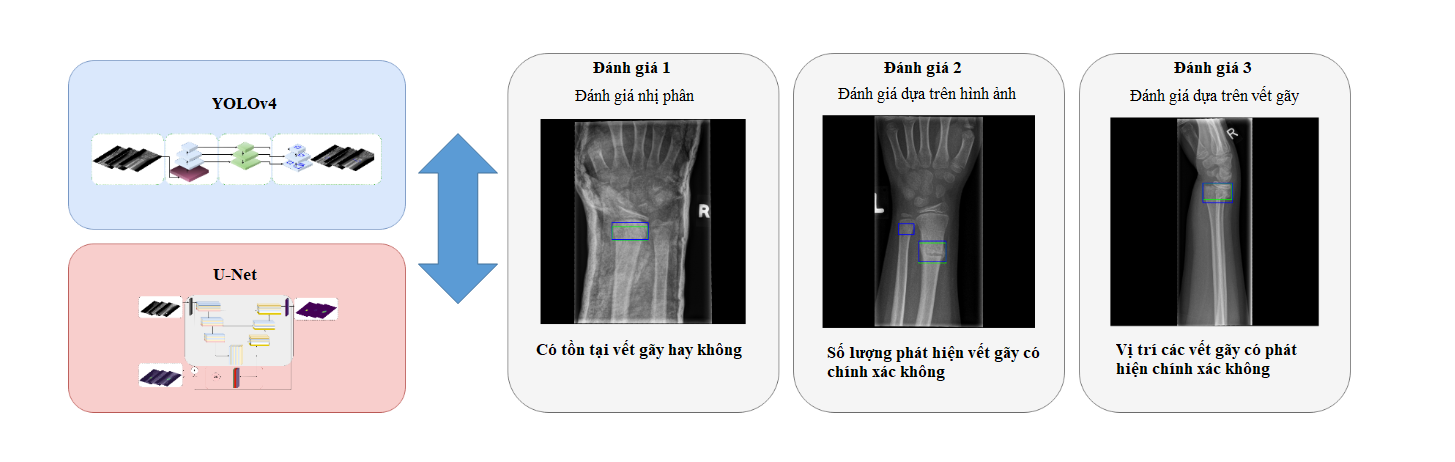
\includegraphics[width=1\textwidth]{images/eval.png}
		\caption{Minh họa về quy trình đánh giá mô hình.}
		\label{fig:model_eval}
	\end{figure}

	Hình \ref{fig:model_eval} mô tả một bản tóm tắt của quá trình đánh giá mô hình được thực hiện trong luận văn này.



}


\end{document}